%%%%%%%%%%%%%%%%%%%%%%%%%%%%%%%%%%%%%%%%%
% Beamer Presentation
% LaTeX Template
% Version 2.0 (March 8, 2022)
%
% This template originates from:
% https://www.LaTeXTemplates.com
%
% Author:
% Vel (vel@latextemplates.com)
%
% License:
% CC BY-NC-SA 4.0 (https://creativecommons.org/licenses/by-nc-sa/4.0/)
%
%%%%%%%%%%%%%%%%%%%%%%%%%%%%%%%%%%%%%%%%%

%----------------------------------------------------------------------------------------
%	PACKAGES AND OTHER DOCUMENT CONFIGURATIONS
%----------------------------------------------------------------------------------------

\documentclass[
	10pt, % Set the default font size, options include: 8pt, 9pt, 10pt, 11pt, 12pt, 14pt, 17pt, 20pt
	%t, % Uncomment to vertically align all slide content to the top of the slide, rather than the default centered
	%aspectratio=169, % Uncomment to set the aspect ratio to a 16:9 ratio which matches the aspect ratio of 1080p and 4K screens and projectors
	hmargin=1cm,vmargin=0cm,head=0.5cm,headsep=0pt,foot=0.5cm,margin=2cm
]{beamer}

% Hide navigation symbols
\setbeamertemplate{navigation symbols}{}

\usepackage{caption}
\captionsetup[figure]{labelsep=space}
\renewcommand{\figurename}{}
\renewcommand{\tablename}{}
\graphicspath{{images/}{./}} % Specifies where to look for included images (trailing slash required)
% \usepackage{minted}
\usepackage{amsmath}
\usepackage{multirow}
\usepackage{color, colortbl}
\usepackage{xcolor}
\usepackage{booktabs} % Allows the use of \toprule, \midrule and \bottomrule for better rules in tables
\usepackage{graphicx}
\usepackage{minibox}
\renewcommand{\arraystretch}{1.2} % Default value: 1
\definecolor{darkGreen}{RGB}{9,150,3} 
\usepackage{tikz}


\newcommand{\tikzunderarrow}[2][black]{\tikz[baseline={(N.base)}]{
  \node[inner sep=0, outer sep=0](N) {#2};
  \draw[overlay, -latex, line width=.04em, #1]
    ([yshift=-.14em]N.south west) -- ([yshift=-.14em]N.south east);}}
% \usepackage[margin=2cm]{geometry}
% \usepackage[most]{tcolorbox}
% \newtcolorbox{mytextbox}[1][]{%
%   sharp corners,
%   enhanced,
%   colback=white,
%   height=10cm,
%   attach title to upper,
%   #1
% }
%----------------------------------------------------------------------------------------
%	SELECT LAYOUT THEME
%----------------------------------------------------------------------------------------
%
% Beamer comes with a number of default layout themes which change the colors and layouts of slides. Below is a list of all themes available, uncomment each in turn to see what they look like.

%\usetheme{default}
%\usetheme{AnnArbor}
%\usetheme{Antibes}
%\usetheme{Bergen}
%\usetheme{Berkeley}
% \usetheme{Berlin}
%\usetheme{Boadilla}
% \usetheme{CambridgeUS}
% \usetheme{Copenhagen}
% \usetheme{Darmstadt}
% \usetheme{Dresden}
% \usetheme{Frankfurt}
% \usetheme{Goettingen}
% \usetheme{Hannover}
% \usetheme{Ilmenau}
% \usetheme{JuanLesPins}
% \usetheme{Luebeck}
\usetheme{Madrid}
%\usetheme{Malmoe}
%\usetheme{Marburg}
%\usetheme{Montpellier}
%\usetheme{PaloAlto}
%\usetheme{Pittsburgh}
%\usetheme{Rochester}
%\usetheme{Singapore}
%\usetheme{Szeged}
%\usetheme{Warsaw}

%----------------------------------------------------------------------------------------
%	SELECT COLOR THEME
%----------------------------------------------------------------------------------------

% Beamer comes with a number of color themes that can be applied to any layout theme to change its colors. Uncomment each of these in turn to see how they change the colors of your selected layout theme.

% \usecolortheme{albatross}
% \usecolortheme{beaver}
% \usecolortheme{beetle}
% \usecolortheme{crane}
% \usecolortheme{dolphin}
% \usecolortheme{dove}
% \usecolortheme{fly}
% \usecolortheme{lily}
% \usecolortheme{monarca}
% \usecolortheme{seagull}
% \usecolortheme{seahorse}
\usecolortheme{spruce}
% \usecolortheme{whale}
% \usecolortheme{wolverine}

%----------------------------------------------------------------------------------------
%	SELECT FONT THEME & FONTS
%----------------------------------------------------------------------------------------

% Beamer comes with several font themes to easily change the fonts used in various parts of the presentation. Review the comments beside each one to decide if you would like to use it. Note that additional options can be specified for several of these font themes, consult the beamer documentation for more information.

\usefonttheme{default} % Typeset using the default sans serif font
%\usefonttheme{serif} % Typeset using the default serif font (make sure a sans font isn't being set as the default font if you use this option!)
\usefonttheme{structurebold} % Typeset important structure text (titles, headlines, footlines, sidebar, etc) in bold
%\usefonttheme{structureitalicserif} % Typeset important structure text (titles, headlines, footlines, sidebar, etc) in italic serif
%\usefonttheme{structuresmallcapsserif} % Typeset important structure text (titles, headlines, footlines, sidebar, etc) in small caps serif

%------------------------------------------------

%\usepackage{mathptmx} % Use the Times font for serif text
\usepackage{palatino} % Use the Palatino font for serif text

%\usepackage{helvet} % Use the Helvetica font for sans serif text
\usepackage[default]{opensans} % Use the Open Sans font for sans serif text
%\usepackage[default]{FiraSans} % Use the Fira Sans font for sans serif text
%\usepackage[default]{lato} % Use the Lato font for sans serif text

%----------------------------------------------------------------------------------------
%	SELECT INNER THEME
%----------------------------------------------------------------------------------------

% Inner themes change the styling of internal slide elements, for example: bullet points, blocks, bibliography entries, title pages, theorems, etc. Uncomment each theme in turn to see what changes it makes to your presentation.

%\useinnertheme{default}
\useinnertheme{circles}
% \useinnertheme{rectangles}
% \useinnertheme{rounded}
%\useinnertheme{inmargin}

%----------------------------------------------------------------------------------------
%	SELECT OUTER THEME
%----------------------------------------------------------------------------------------

% Outer themes change the overall layout of slides, such as: header and footer lines, sidebars and slide titles. Uncomment each theme in turn to see what changes it makes to your presentation.

% \useoutertheme{default}
% \useoutertheme{infolines}
\useoutertheme{miniframes}
% \useoutertheme{smoothbars}
% \useoutertheme{sidebar}
%\useoutertheme{split}
% \useoutertheme{shadow}
% \useoutertheme{tree}
%\useoutertheme{smoothtree}
%----------------------------------------------------------------------------------------
%	PRESENTATION INFORMATION
%----------------------------------------------------------------------------------------

\title[LAB 03: Integer Arithmetic]{LAB 03: Integer Arithmetic} % The short title in the optional parameter appears at the bottom of every slide, the full title in the main parameter is only on the title page

\author[S. AlSaleh]{Saleh AlSaleh \\ \smallskip \textit{salehs@kfupm.edu.sa}} % Presenter name(s), the optional parameter can contain a shortened version to appear on the bottom of every slide, while the main parameter will appear on the title slide

\institute[KFUPM]{King Fahd University of Petroleum and Minerals \\ College of Computing and Mathematics \\ Computer Engineering Department} % Your institution, the optional parameter can be used for the institution shorthand and will appear on the bottom of every slide after author names, while the required parameter is used on the title slide and can include your email address or additional information on separate lines

\date[January 29, 2023]{COE301: Computer Architecture \\ Term 222} % Presentation date or conference/meeting name, the optional parameter can contain a shortened version to appear on the bottom of every slide, while the required parameter value is output to the title slide

%----------------------------------------------------------------------------------------

\begin{document}

%----------------------------------------------------------------------------------------
%	TITLE SLIDE
%----------------------------------------------------------------------------------------

\begin{frame}
	% Output the title slide, automatically created using the text entered in the PRESENTATION INFORMATION block above
	\titlepage
\end{frame}

%----------------------------------------------------------------------------------------
%	TABLE OF CONTENTS SLIDE
%----------------------------------------------------------------------------------------

\begin{frame}
	\frametitle{Agenda} % Slide title, remove this command for no title
	\tableofcontents % Output the table of contents (all sections on one slide)
\end{frame}

%----------------------------------------------------------------------------------------
%	PRESENTATION BODY SLIDES
%----------------------------------------------------------------------------------------

\section{Overflow} 
\begin{frame}
	\frametitle{Overflow}
	
	\begin{itemize}
		\item Max positive integer number represented in  4-bit: \pause \( (+7)_{10} = (0111)_2 \) \pause
		\item Min negative integer number represented in  4-bit: \pause \( (-8)_{10} = (1000)_2 \) \pause  
		\item Max positive integer number represented in 32-bit: \pause \( (0x7FFFFFFF)_{16} \)  \pause
		\item Min negative integer number represented in 32-bit: \pause \( (0x80000000)_{16} \)  \pause
		\item add/sub causes/raises arithmetic exception in the case of overflow and result is not written. \pause
		\item addu/subu ignores overflow and writes result to destination register
	\end{itemize}
\end{frame}

\section{Logical Bitwise Instructions} 
\begin{frame}
	\frametitle{Logical Bitwise Instructions}
	\begin{columns}[c]
		
		\begin{column}{0.45\textwidth} 
			\begin{columns}[c]
				\begin{column}{0.3\textwidth} 
					\begin{figure}
						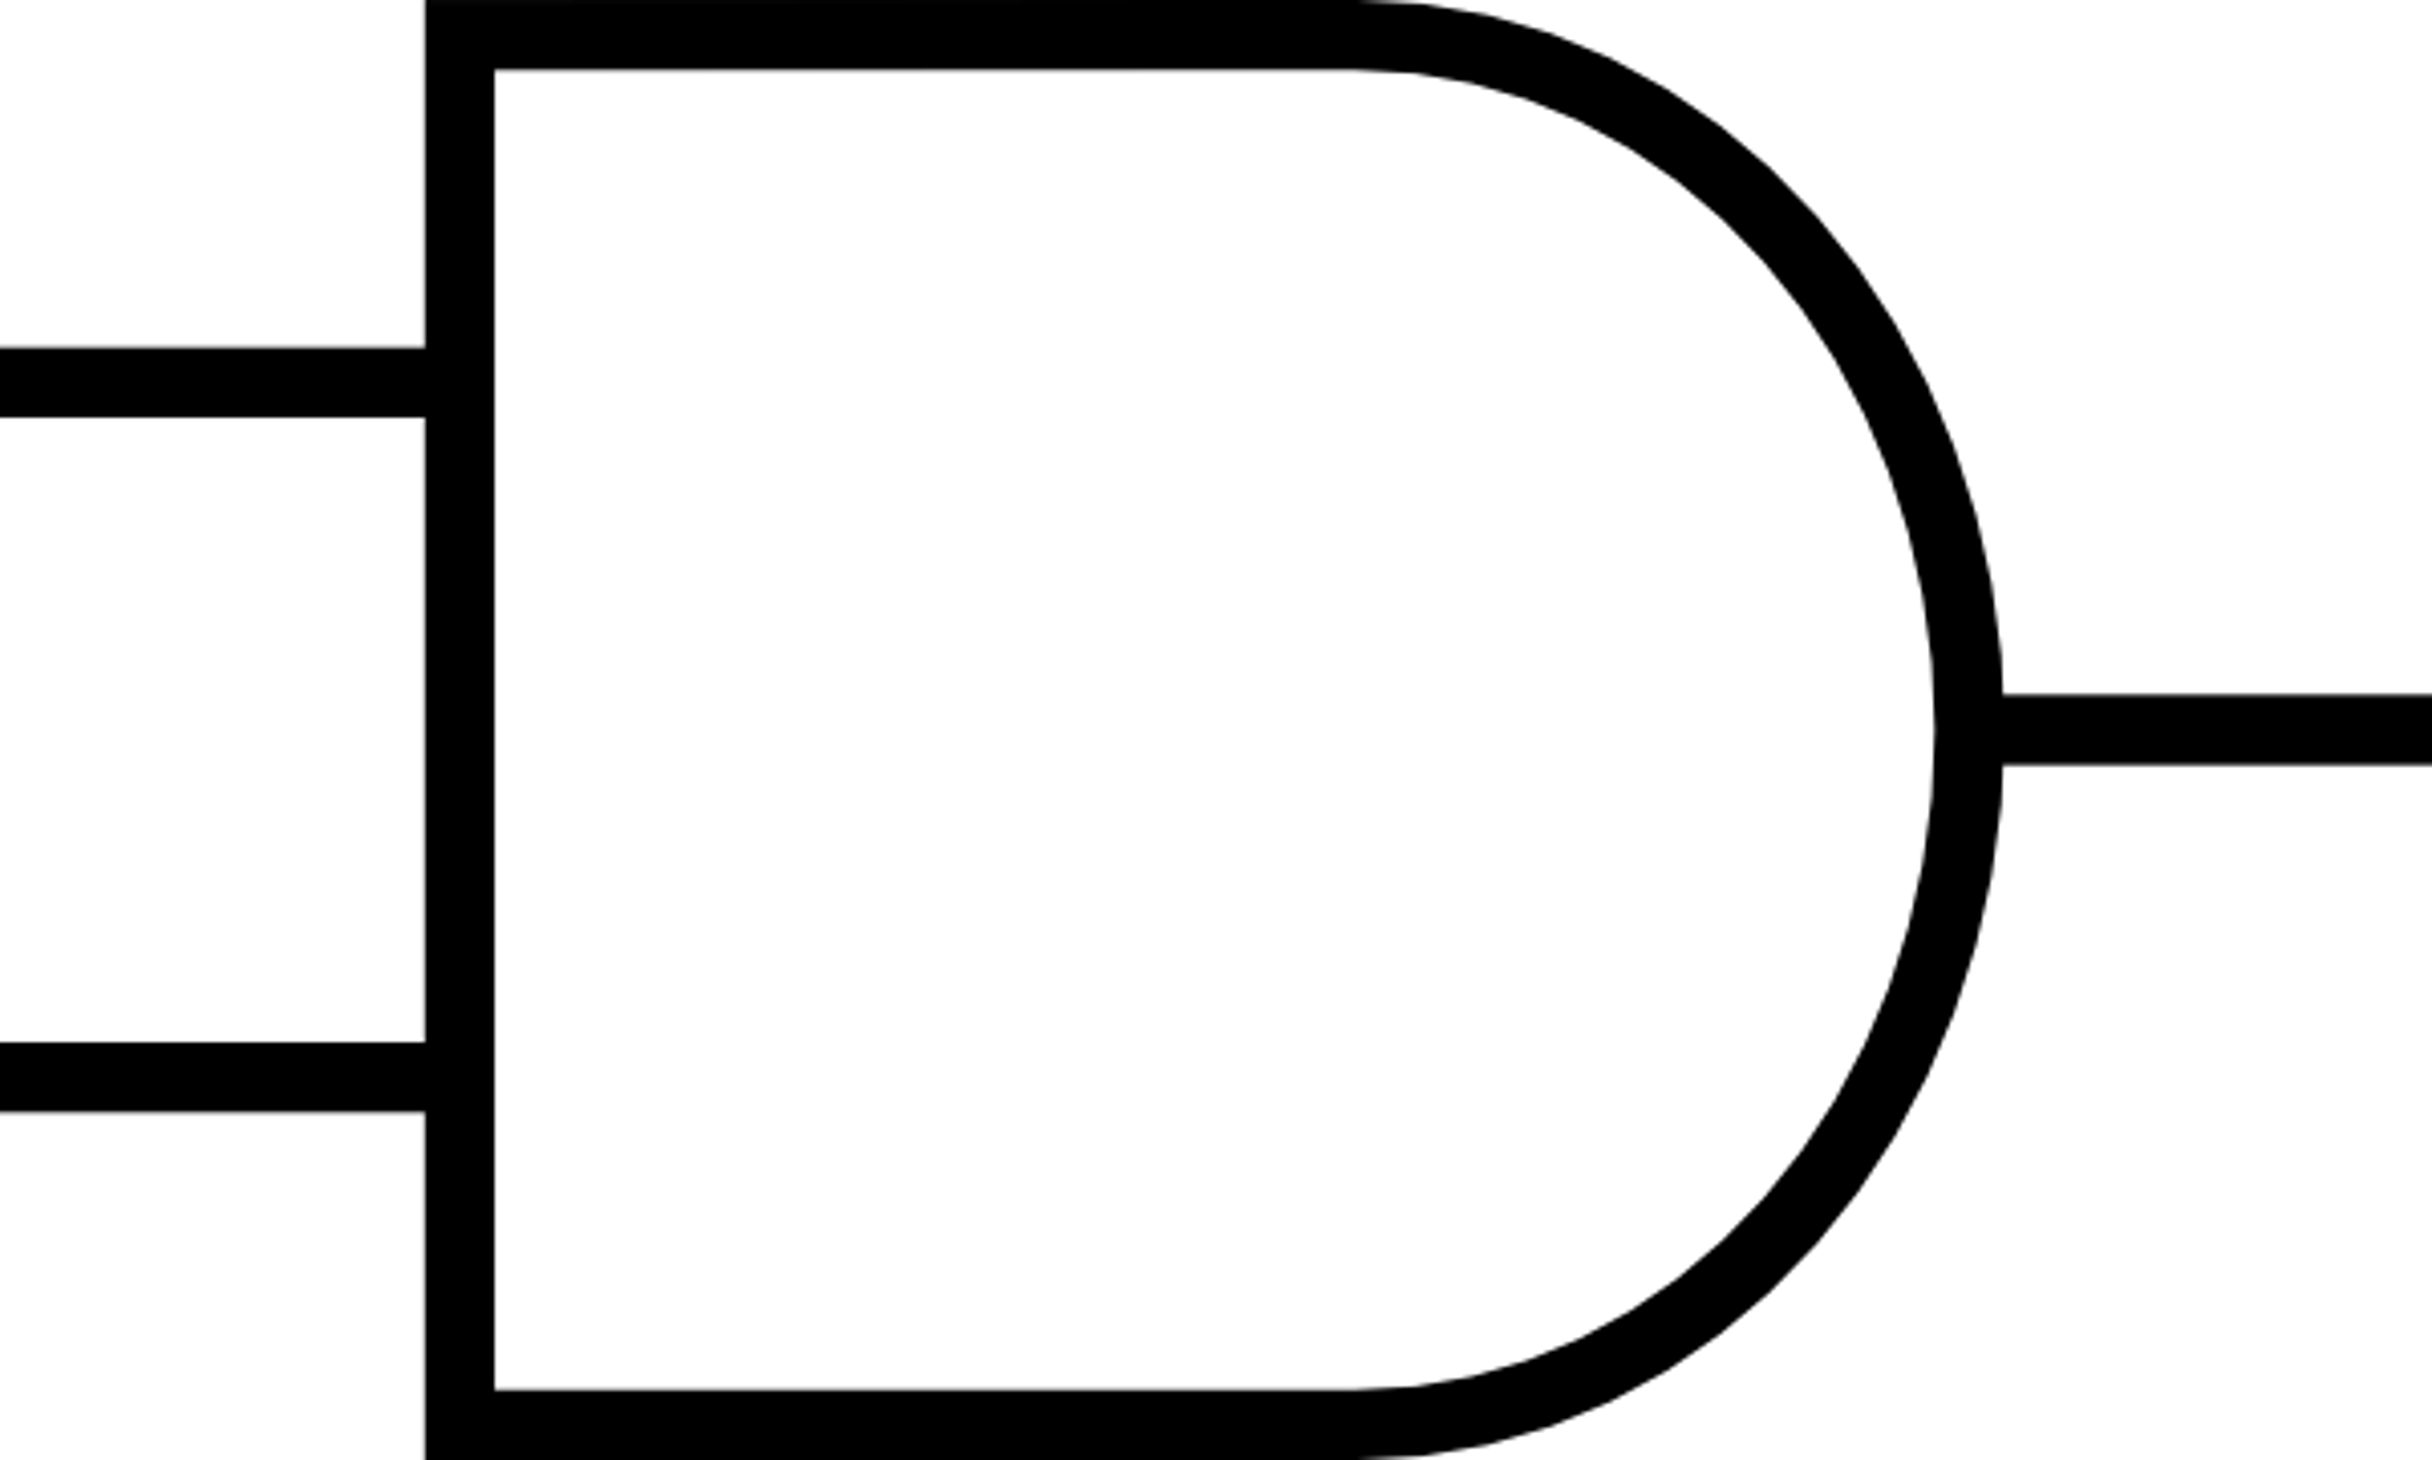
\includegraphics[width=0.7\textwidth]{and.png}
						\caption{AND}
					\end{figure}
				\end{column}
				\begin{column}{0.7\textwidth} 
					\begin{table}
						\resizebox{\linewidth}{!}{%
						\begin{tabular}{c|c|c|c|c}
											& \( b_3 \) & \( b_2 \) & \( b_1 \) & \( b_0 \) \\ 
							\toprule
							A 				& 0 		& 1			& 0			& 1			\\
							B 				& 1 		& 1			& 0			& 0			\\ 
							\bottomrule
							\( A \& B \) 	& 0 		& 1			& 0			& 0 		\\
						\end{tabular}%
						}
					\end{table}
				\end{column}
			\end{columns}
			\pause
			\begin{columns}[c]
				\begin{column}{0.3\textwidth} 
					\begin{figure}
						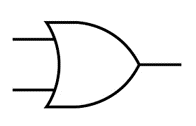
\includegraphics[width=0.7\textwidth]{or.png}
						\caption{OR}
					\end{figure}
				\end{column}
				\begin{column}{0.7\textwidth} 
					\begin{table}
						\resizebox{\linewidth}{!}{%
						\begin{tabular}{c|c|c|c|c}
											& \( b_3 \) & \( b_2 \) & \( b_1 \) & \( b_0 \) \\ 
							\toprule
							A 				& 0 		& 1			& 0			& 1			\\
							B 				& 1 		& 1			& 0			& 0			\\ 
							\bottomrule
							\( A | B \) 	& 1 		& 1			& 0			& 1 		\\
						\end{tabular}%
						}
					\end{table}
				\end{column}
			\end{columns}
		\end{column}

		

		\begin{column}{0.45\textwidth} 
			\pause
			\begin{columns}[c]
				\begin{column}{0.3\textwidth} 
					\begin{figure}
						
\includegraphics[width=0.7\textwidth]{xor.png}
						\caption{XOR}
					\end{figure}
				\end{column}
				\begin{column}{0.7\textwidth} 
					\begin{table}
						\resizebox{\linewidth}{!}{%
						\begin{tabular}{c|c|c|c|c}
												& \( b_3 \) & \( b_2 \) & \( b_1 \) & \( b_0 \) \\ 
							\toprule
							A 					& 0 		& 1			& 0			& 1			\\
							B 					& 1 		& 1			& 0			& 0			\\ 
							\bottomrule
							\( A \land B \) 	& 1 		& 0			& 0			& 1 		\\
						\end{tabular}%
						}
					\end{table}
				\end{column}
			\end{columns}
			\pause
			\begin{columns}[c]
				\begin{column}{0.3\textwidth} 
					\begin{figure}
						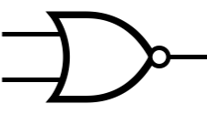
\includegraphics[width=0.7\textwidth]{nor.png}
						\caption{NOR}
					\end{figure}
				\end{column}
				\begin{column}{0.7\textwidth} 
					\begin{table}
						\resizebox{\linewidth}{!}{%
						\begin{tabular}{c|c|c|c|c}
														& \( b_3 \) & \( b_2 \) & \( b_1 \) & \( b_0 \) \\ 
							\toprule
							A 							& 0 		& 1			& 0			& 1			\\
							B 							& 1 		& 1			& 0			& 0			\\ 
							\bottomrule
							\( \overline{(A | B)} \) 	& 0 		& 0			& 1			& 0 		\\
						\end{tabular}%
						}
					\end{table}
				\end{column}
			\end{columns}
		\end{column}
	\end{columns}
\end{frame}

\section{Shift Instructions} 

\begin{frame}
	\frametitle{Shift Instructions (Left Shift)}
	\begin{columns}[c]
		\begin{column}{0.2\textwidth}
			\hspace{0.5cm} \( (0010)_2 \) \\ \pause
			\hspace{0.9cm} 2
		\end{column}

		\begin{column}{0.6\textwidth}
			\tikzunderarrow{Shift every bit to the left by 1}
			\\ and append 0 in the LSB 
			\pause
		\end{column}

		\begin{column}{0.2\textwidth}
			\hspace{-2cm} \( (010\color{red}0\color{black})_2\) \\
			\hspace{-1.6cm} 4
			\pause
		\end{column}
	\end{columns}
	\vspace{1cm}
	\begin{columns}[c]
		\begin{column}{0.2\textwidth}
			\hspace{0.5cm} \( (0100)_2 \) \\
			\hspace{0.9cm} 4
		\end{column}

		\begin{column}{0.6\textwidth}
			\tikzunderarrow{Shift every bit to the left by 1}
			\\ and append 0 in the LSB 
			\pause
		\end{column}

		\begin{column}{0.2\textwidth}
			\hspace{-2cm} \( (100\color{red}0\color{black})_2\) \\
			\hspace{-1.6cm} 8 \pause
		\end{column}
	\end{columns}
	\vspace{1cm}
	\begin{itemize}
		\item This is called Shift Left Logical (sll).
		\item Every single shift left logical is equivalent to multiplying by 2.
		\item MIPS instruction: \color{blue}sll \color{red}\$dst\color{black}, \color{red}\$src\color{black}, shift\_amount. \\ 
		\hspace{2.1cm} e.g. \color{blue}sll \color{red}\$t0\color{black}, \color{red}\$t1\color{black}, 3 \\ 
		equivalent to multiplying \$t1 by \( 2^3 = 8 \)
	\end{itemize}
\end{frame}

\begin{frame}
	\frametitle{Shift Instructions (Logical Right Shift)}
	\begin{columns}[c]
		\begin{column}{0.2\textwidth}
			\hspace{0.5cm} \( (1010)_2 \) \\ \pause
			\hspace{0.9cm} 10
		\end{column}

		\begin{column}{0.6\textwidth}
			\tikzunderarrow{Shift every bit to the right by 1}
			\\ and append 0 in the MSB 
			\pause
		\end{column}

		\begin{column}{0.2\textwidth}
			\hspace{-2cm} \( (\color{red}0\color{black}101)_2\) \\
			\hspace{-1.6cm} 5
			\pause
		\end{column}
	\end{columns}
	\vspace{1cm}
	\begin{columns}[c]
		\begin{column}{0.2\textwidth}
			\hspace{0.5cm} \( (0101)_2 \) \\
			\hspace{0.9cm} 5
		\end{column}

		\begin{column}{0.6\textwidth}
			\tikzunderarrow{Shift every bit to the right by 1}
			\\ and append 0 in the MSB 
			\pause
		\end{column}

		\begin{column}{0.2\textwidth}
			\hspace{-2cm} \( (\color{red}0\color{black}010)_2\) \\
			\hspace{-1.6cm} 2 \pause
		\end{column}
	\end{columns}
	\vspace{1cm}
	\begin{itemize}
		\item This is called Shift Right Logical (srl).
		\item Every single shift right logical is equivalent to dividing by \color{red} 2 (with floor) \color{black}.
		\item MIPS instruction: \color{blue} srl \color{red}\$dst\color{black}, \color{red}\$src\color{black}, shift\_amount. \\ 
		\hspace{2.1cm} e.g. \color{blue}srl \color{red}\$t0\color{black}, \color{red}\$t1\color{black}, 3 \\ 
		equivalent to dividing (with floor) \$t1 by \( 2^3 = 8 \)
	\end{itemize}
\end{frame}

\begin{frame}
	\frametitle{Shift Instructions (Arithmetic Right Shift)}
	\begin{columns}[c]
		\begin{column}{0.2\textwidth}
			\hspace{0.5cm} \( (1010)_2 \) \\ \pause
			\hspace{0.9cm} -6
		\end{column}

		\begin{column}{0.6\textwidth}
			\tikzunderarrow{Shift every bit to the right by 1}
			\\ and duplicate the sign bit 
			\pause
		\end{column}

		\begin{column}{0.2\textwidth}
			\hspace{-2cm} \( (\color{red}1\color{black}101)_2\) \\
			\hspace{-1.6cm} -3
			\pause
		\end{column}
	\end{columns}
	\vspace{1cm}
	\begin{columns}[c]
		\begin{column}{0.2\textwidth}
			\hspace{0.5cm} \( (1101)_2 \) \\ 
			\hspace{0.9cm} -3
		\end{column}

		\begin{column}{0.6\textwidth}
			\tikzunderarrow{Shift every bit to the right by 1}
			\\ and duplicate the sign bit 
			\pause
		\end{column}

		\begin{column}{0.2\textwidth}
			\hspace{-2cm} \( (\color{red}1\color{black}110)_2\) \\
			\hspace{-1.6cm} -2 \pause
		\end{column}
	\end{columns}
	\vspace{1cm}
	\begin{itemize}
		\item This is called Shift Right Arithmetic (sra).
		\item Every single shift right arithmetic is equivalent to dividing by \color{red}2 (with floor) for \underline{\textbf{signed numbers}}\color{black}.
		\item MIPS instruction: \color{blue}sra \color{red}\$dst\color{black}, \color{red}\$src\color{black}, shift\_amount. \\ 
		\hspace{2.1cm} e.g. \color{blue}sra \color{red}\$t0\color{black}, \color{red}\$t1\color{black}, 3 \\ 
		equivalent to dividing (with floor) \$t1 as a signed number by \( 2^3 = 8 \)
	\end{itemize}
\end{frame}


\section{Pseudo Instructions}
\begin{frame}
	\frametitle{Pseudo Instructions}
	
	\begin{columns}[c]
		
		\begin{column}{0.7\textwidth}
			\begin{itemize}
				\item Maps to one or more basic simple assembly instruction(s). \pause
				\item They ease the programmer's tasks in writing applications. \pause
				\item Common pseudo instructions: li, la, abs. \pause
					\begin{itemize}
						\item \color{blue}li \color{red}\$t0\color{black}, 0xABCD \hspace{0.62cm} \( \Rightarrow \) 	\color{blue}addi \color{red}\$t0\color{black}, \color{red}\$0\color{black}, 0xABCD \pause
						\item \color{blue}li \color{red}\$t0\color{black}, 0x89ABCDEF 	\( \Rightarrow \) 	\color{blue}lui \color{red}\$at\color{black}, 0x89AB \\ 
						\hspace{3.15cm} \color{blue}ori \color{red}\$t0\color{black}, \color{red}\$at\color{black}, 0xCDEF \pause
					\end{itemize}
			\end{itemize}
		\end{column}

		\begin{column}{0.3\textwidth}
			\begin{table}
				\resizebox{\linewidth}{!}{%
				\begin{tabular}{p{0.47\textwidth}|p{0.47\textwidth} p{0.1\textwidth}}
					\begin{tabular}[l]{@{}l@{}}Load\\Upper\\16 bit\end{tabular} 	& \begin{tabular}[l]{@{}l@{}}Clear\\Lower\\16 bit\end{tabular} 	                & \\
					\toprule
					0x89AB 				 & 0x0000 								& \vline \color{red}\$at \\ \hline
					0x89AB 				 & 0xCDEF 								& \vline \color{red}\$t0 \\
					\bottomrule
					\begin{tabular}[l]{@{}l@{}}Keep\\Upper\\16 bit\end{tabular} 	& \begin{tabular}[l]{@{}l@{}}OR Lower\\16 bit with\\immediate\\value\end{tabular}  	& \\
				\end{tabular}%
				}
			\end{table}
		\end{column}


	\end{columns}
\end{frame}


\section{Live Examples}

\begin{frame}
	\frametitle{Live Examples}
	
\end{frame}

%------------------------------------------------

\section{Tasks}

\begin{frame}
	\frametitle{Task \#1}
	Write a MIPS program where you ask the user to enter a \underline{\textbf{signed integer x}}.

	Then, calculate and print the value of \textbf{y} based on the following equation.
	\begin{equation*}
		y = 53.125 x
	\end{equation*}


	\begin{columns}[c]
		\begin{column}{0.2\textwidth}
			Sample Run 1

			\minibox[frame,pad=8pt]{
				\color{black} Enter x: \color{blue} 8 \\
				\color{black} y = \color{darkGreen} 425 \\
			}	
		\end{column}
		\begin{column}{0.2\textwidth}
			Sample Run 2

			\minibox[frame,pad=8pt]{
				\color{black} Enter x: \color{blue} -16 \\
				\color{black} y = \color{darkGreen} -850 \\
			}		
		\end{column}
	\end{columns}
\end{frame}

\begin{frame}
	\frametitle{Task \#2}
	Write a MIPS program where you prompt the user for an integer \textbf{a}.

	Then, set bit 11 and 17. Finally, display the value of that integer after modification. \newline	
	
	

	\begin{columns}[c]
		\begin{column}{0.2\textwidth}
			Sample Run 1

			\minibox[frame,pad=8pt]{
				\color{black} Enter a: \color{blue} 465  \\
				\color{black} Result = \color{darkGreen} 133585 \\
			}	
		\end{column}
		\begin{column}{0.2\textwidth}
			Sample Run 2

			\minibox[frame,pad=8pt]{
				\color{black} Enter a: \color{blue} 1023 \\
				\color{black} Result = \color{darkGreen} 134143 \\
			}		
		\end{column}
	\end{columns}
\end{frame}

%----------------------------------------------------------------------------------------

\end{document} 
